\documentclass[a4paper,twocolumn,10pt]{article}
%\usepackage[spanish]{babel}
%\usepackage[latin1]{inputenc}
\usepackage{graphicx}
\usepackage{flushend}
\usepackage[T1]{fontenc}
\usepackage{helvet}%arial
\renewcommand{\familydefault}{\sfdefault}
\usepackage[utf8]{inputenc}%acentos sin codigo
\usepackage[spanish,es-tabla]{babel} %tablas no cuadros
\parindent=0.7cm %sangria % ojo
\usepackage{amsmath} %simbolos matematicos
\usepackage{amssymb,amsfonts,latexsym,cancel}
\usepackage{array}
\usepackage{bm} %negritas
\usepackage{float} %ubicar figuras
\usepackage{fancyhdr} %darle formato al documento
\usepackage{graphicx}
\usepackage{multirow}
\usepackage{subfig}
\usepackage{geometry}
\usepackage{siunitx}

%Comandos que yo agregue
\usepackage{comment}
\newcommand{\grad}{$^{\circ}$ }
\usepackage{booktabs}
\usepackage{amssymb}% http://ctan.org/pkg/amssymb
\usepackage{pifont}% http://ctan.org/pkg/pifont

\geometry{
	lmargin=2cm,rmargin=2cm,top=1cm,bottom=2cm,includeheadfoot}
\usepackage{titlesec}
\titleformat*{\section}{\small\bfseries\sffamily}
\titleformat*{\subsection}{\small\bfseries\sffamily}
\titleformat*{\subsubsection}{\small\bfseries\sffamily}
\titleformat*{\paragraph}{\small\bfseries\sffamily}

\usepackage{fancyhdr}
\pagestyle{fancy}
\lhead{}
\chead{Implementación de un ChatBot utilizando algoritmos de Inteligencia Artificial.}
\rhead{}
\lfoot{Facultad de Ingeniería -- UNA}
\rfoot{Mayo, 2023}
%\renewcommand{\footrulewidth}{1.5pt}

\fancypagestyle{firststyle}
{
	\fancyhf{}
	\fancyfoot[C]{\footnotesize \thepage}
	\fancyfoot[L]{Facultad de Ingeniería -- UNA}
	\fancyfoot[R]{Mayo, 2023}
	\fancyhead[L]{
\includegraphics[height=1.5cm]{Figuras/Fiuna.png}}
	\fancyhead[R]{
\includegraphics[height=1.5cm]{Figuras/Logo_UNA.jpg}}
	\fancyhead[C]{Resumen Técnico\\ \text{}}
	%\renewcommand{\footrulewidth}{1.5pt}

}
\renewcommand{\headrulewidth}{1.5pt}
%\usepackage{graphicx}
%\setlength{\columnsep}{distance}
\usepackage{multicol}
%\thispagestyle{firststyle}
%\usepackage{microtype}
%\usepackage{vwcol}

%\usepackage{tabularx}
%    \newcolumntype{L}{>{\raggedright\arraybackslash}X}

\usepackage[normalem]{ulem}

\usepackage[labelfont=bf]{caption}

\usepackage{authblk}
\renewcommand\Authands{, }
%\renewcommand{\lastandname}{\unskip}

%\normalsize
\renewcommand\Affilfont{\fontsize{8}{10.8}\itshape}
\begin{document}

\title{\large Implementación de un ChatBot utilizando algoritmos de Inteligencia Artificial.}
%\author[3]{Msc. Enrique G. Paiva}
%\author[3]{Dr. Diego H. Stalder}
%\author[3]{Msc. Sergio R. Toledo}
\author[1]{Carlos Buenaventura Ozuna Loncharich}
\author[2]{Oscar Bartolome Valdez Sarubbi}
\author[3]{Prof. Ing. Aurora Nuñez }


\affil[1]{Alumno, Facultad de Ingeniería. Universidad Nacional de Asunción. San Lorenzo, Paraguay}
\affil[2]{Alumno, Facultad de Ingeniería. Universidad Nacional de Asunción. San Lorenzo, Paraguay}
\affil[3]{Orientadora, Facultad de Ingeniería. Universidad Nacional de Asunción. San Lorenzo, Paraguay}
%\affil[1]{Alumno, ovaldez@ing.una.py, Facultad de Ingeniería. Universidad Nacional de
%	Asunción. San Lorenzo, Paraguay}
%\affil[2]{Alumno, guille94arguello@gmail.com, Facultad de Ingeniería. Universidad Nacional de
%	Asunción. San Lorenzo, Paraguay}
%\affil[3]{Orientador, Facultad de Ingeniería. Universidad Nacional de Asunción. San Lorenzo,
%	Paraguay}

\date{}
%\vspace{-5cm}

%TODO: agregar contenido en el mismo formato
\twocolumn[
	\begin{@twocolumnfalse}
		\maketitle
		%%\hline \\
		%\hspace{-0.5cm} \rule{\linewidth}{0.1mm}\\
		%\begin{table}
		\centering
		\begin{tabular}{p{6cm} p{10.3cm}} %4.3 12
			\\ \hline

			\vspace{-0.1cm}
			\uline{Palabras clave:\hfill}
			\begin{itemize}
				\setlength\itemsep{-0.2em}
				\item Sistemas de Determinación y Control de Actitud (ADCS)
				\item Magnetorquer
				\item Rueda de reacción
				\item Jaula de Helmholtz
			\end{itemize}
			                                                        & \vspace{-0.1cm}
			\uline{Resumen\hfill}
			\thispagestyle{firststyle}

			El Sistema de Determinación y Control de Actitud (ADCS) es un subsistema
			crucial de un satélite CubeSat, ya que proporciona precisión y estabilidad de puntería para las
			cargas útiles y las antenas, utilizando sensores para determinar y actuadores para controlar la
			actitud. El presente Trabajo Final de Grado presenta el diseño e implementación de un modelo
			conceptual ADCS para un CubeSat de 1-U. Son implementados,  el algoritmo del filtro Madgwick para
			determinar la actitud a partir de una representación de cuaterniones, y el método de compensación
			PID para controlar a los actuadores. El primer paso para diseñar es definir los marcos de
			referencia, la representación de la actitud y los algortimos ADCS. Así también se diseñan los
			distintos dispositivos que componen el hardware del ADCS con la estructura del CubeSat, que
			finalmente son implementados mediante la integración completa, realizando validaciones de
			funcionamiento a través de simulaciones y pruebas experimentales en un banco de pruebas construido,
			consistiendo en una jaula de Helmholz de 1 eje y la denominada prueba piñata. El diseño e
			implementación del modelo conceptual del ADCS con la jaula de Hemholtz apoyan a el desarrollo de
			capacidades y la educación en ingeniería espacial en las universidades paraguayas

			\text{}
			\\
			\uline{Keywords\hfill}
			\begin{itemize}
				\setlength\itemsep{-0.2em}
				\item Attitude Determination and Control Systems (ADCS)
				\item Magnetorquer
				\item Reaction wheel
				\item Helmholtz cage
			\end{itemize} &
			\uline{Abstract \hfill}

			The Attitude Determination and Control System (ADCS) is a crucial subsystem
			of a CubeSat satellite, providing precision and pointing stability for payloads and antennas, using
			sensors to determine and actuators to control attitude. This Final Degree Project presents the
			design and implementation of an ADCS conceptual model for a 1-U CubeSat. They are implemented, the
			Madgwick filter algorithm to determine the attitude from a representation of quaternions, and the
			PID compensation method to control the actuators. The first step in designing is to define the
			frames of reference, the attitude representation, and the ADCS algorithms. Also the different
			devices that compose the ADCS hardware are designed with the CubeSat structure, which are finally
			implemented through complete integration, performing operational validations through simulations
			and experimental tests on a built test bench, consisting of a cage. Helmholtz 1 axis and the
			so-called piñata test. The design and implementation of the ADCS conceptual model with the
			Helmholtz cage support capacity development and education in space engineering in Paraguayan
			universities.

			\\ \hline

		\end{tabular}

		%\hspace{-0.5cm} \rule{\linewidth}{0.1mm}\\
	\end{@twocolumnfalse}
]
%ozuna

\section{Introducción}
La Inteligencia Artificial (IA) ha tenido un crecimiento exponencial en los últimos años debido a la capacidad de cómputo asequible y de alto rendimiento, así como a la disponibilidad de grandes volúmenes de datos. Se destaca el Procesamiento de Lenguaje Natural (PLN) como una de las áreas de estudio de la IA que utiliza modelos estadísticos, aprendizaje automático y aprendizaje profundo para permitir que las computadoras entiendan e interpreten el lenguaje humano.\\
\indent Una de las tantas aplicaciones prácticas del PLN son los chatbots, programas que imitan la conversación humana y son capaces de interactuar con personas y responder adecuadamente a sus preguntas. Los chatbots son accesibles, eficientes y de alta disponibilidad, lo que permite que diferentes industrias se beneficien de ellos, como el comercio electrónico, los seguros y el cuidado de la salud.\\
\indent El trabajo presenta un chatbot específicamente diseñado para el sector de la educación, con el objetivo de permitir que los estudiantes realicen consultas sobre la Facultad de Ingeniería y obtengan respuestas mediante técnicas de coincidencia de patrones.

\subsection{Objetivo General}

Desarrollar e implementar un Chatbot utilizando algoritmos de Inteligencia Artificial (IA).

\subsection{Objetivos Específicos}
\begin{itemize}
\item Comparar distintas Tecnologías para abordar el problema.
\item Orientar el chatbot a dudas comunes de los estudiantes de la Facultad de Ingeniería en atención al alumno.
\item Recopilar, procesar y filtrar preguntas frecuentes para contar con un dataset
propio.
\item Seleccionar, entrenar y probar el algoritmo utilizando el dataset generado.
\item Implementar el chatbot para su uso por estudiantes de la Facultad de Ingeniería
\item Agregar una interfaz, propia o a una ya existente para el uso por los alumnos.

\end{itemize}

\subsection{Alcance y limitaciones}

Se pretende desarrollar un Chatbot que utilice algoritmos de inteligencia artificial para responder a preguntas frecuentes de los alumnos de la Facultad de Ingeniería de la
UNA. El entrenamiento de la IA se llevará a cabo utilizando un dataset propio en
conjunto con otros ya existentes. Una previa comparativa entre distintas librerías
y plataformas es necesaria para escoger la mejor solución al objetivo planteado.%ozuna


\section{Marco Teórico} %O marco Teórico, que se yo
El Procesamiento de Lenguaje Natural (NPL por sus siglas en inglés) es un campo de las Ciencias de Computación y la Lingüística que trata con métodos para analizar, modelar y entender el lenguaje humano.\\
\begin{figure}[H]
\begin{centering}
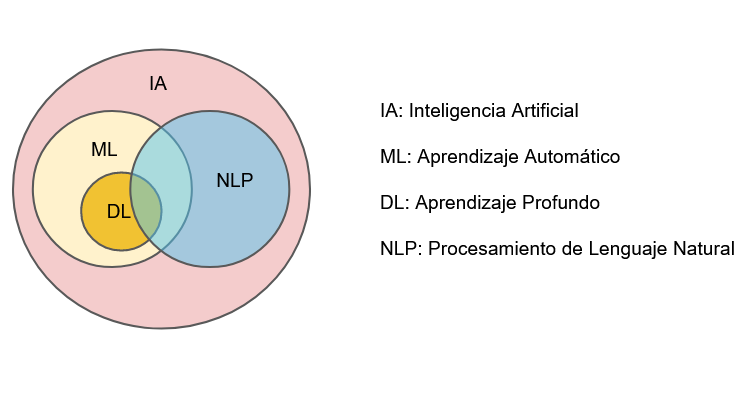
\includegraphics[angle=0,width=0.3\textwidth]{Figuras/NLP.png}
\par \end{centering}
\caption[Procesamiento de Lenguaje Natural]{Procesamiento de Lenguaje Natural. \textbf{Fuente:} Propia}
\label{NLP}
\end{figure}

Existen varios métodos utilizados a lo largo de la historia del Procesamiento de Lenguaje Natural.\\
Los primeros intentos fueron mediante reglas de acciones manuales por medio de árboles de decisión, conocidos como métodos heurísticos o basados en reglas. Este método requiere que los desarrolladores tengan experiencia en el dominio del problema para formular las reglas que puedan ser incorporadas al programa, utilizan bastante los diccionarios y las expresiones regulares.\\
\indent Posteriormente vinieron los métodos basados en aprendizaje automático, como la clasificación y regresión, que son utilizados con frecuencia en NLP.\\
\indent Finalmente, el Aprendizaje profundo o Deep learning(DL), una evolución más compleja de los algoritmos de ML convencionales trajeron nuevas oportunidades al Procesamiento de Lenguaje Natural, un claro ejemplo son las Redes Neuronales Recurrentes (RNN)que están específicamente diseñadas para mantener un procesamiento secuencial y memoria de los pasos anteriores. Esta memoria es temporal, la información es almacenada y actualizada en cada paso de lectura de la RNN. Las RNNs son poderosas y funcionan muy bien en la clasificación de textos, reconocimiento de entidades, traducción automática, y pueden utilizarse para generar textos, por ejemplo para predecir la siguiente palabra a escribirse de acuerdo al contexto de la conversación. A pesar de su versatilidad y capacidad, las RNNs sufren de ciertas limitaciones por contar con memoria temporal, por lo tanto no se desempeñan óptimamente
para textos con largos contextos.\\
\indent Las Redes Neuronales Convencionales (CNN)s también vieron éxito en NLP, específicamente en la clasificación de texto. Se puede reemplazar una palabra de una oración de un texto por un vector palabra, y estos a su vez son colocados en una matriz para poder ser tratados de manera similar a una imagen.\\
\indent Los transformadores son la última innovación en lo que respecta a modelos basados en DL para NLP. Los modelos de transformadores obtuvieron avances en la mayoría de las tareas de NLP en los últimos años. Estos modelan el contexto textual pero no de manera secuencial. Dada una palabra en una entrada de texto, se prefiere mirar las demás palabras vecinas en el texto y representar cada palabra de acuerdo al contexto de las demás.
\begin{figure}[H]
\begin{centering}
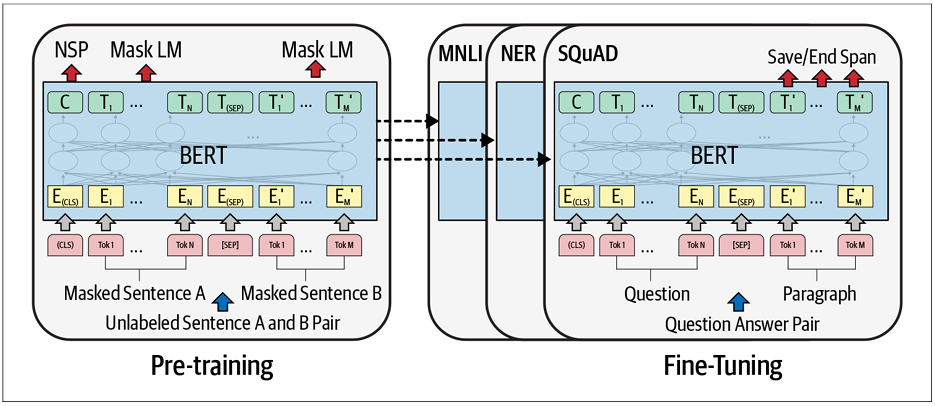
\includegraphics[angle=0,width=0.3\textwidth]{Figuras/tranformers.png}
\par \end{centering}
\caption[Transformadores]{Transformadores. \textbf{Fuente:} \cite{sowmya_practical_npl}}
\label{NLP}
\end{figure}

\subsection{Chatbots}
Los chatbots son programas que imitan la conversación humana utilizando la Inteligencia Artificial.\cite{UniversityRelatedFAQS}
\subsubsection{Características de un Chatbot}
Todos los chatbots deben contar con las siguientes cualidades. \cite{evaluating_quality}
\begin{itemize}
    \item Rendimiento: se refiere a la eficiencia en la asignación de funciones y a la robustez que tienen en cuanto a la manipulación y a las entradas inesperadas.
    \item Funcionalidad: es capaz de interpretar, responder y ejecutar  correctamente las tareas demandadas.
    \item Humanidad: la conversación con el chatbot debe ser natural, lo más parecida a la humana.
    \item Ética: genera confianza, respeta y protege la dignidad, y la privacidad de los usuarios.
    \item Accesibilidad: se encuentra disponible cuando el usuario quiera usarlo, además se refiere a que es capaz de detectar intenciones y significados
\end{itemize}
\subsubsection{Plataformas de desarrollo}
\subsection{Plataformas de desarrollo}
\begin{itemize}
    \item \textbf{DialogFlow:}
        Es la plataforma de desarrollo de chatbots de Google, permite una fácil integración a aplicaciones móviles y web, también facilita bastante el diseño de la interfaz de usuario.\\
        Admite como entrada texto y voz, es capaz de responder a los clientes con texto o voz sintética.\\\cite{Dialogflow}
    \item \textbf{IBM Watson:}
        IBM Watson  permite a los usuarios integrar sus chatbots en cualquier canal, sea web, aplicaciones o incluso una llamada.\\
        Es capaz de aprender los vocabularios de la industria,  términos coloquiales o dialectos regionales, admite entradas de voz y también de texto. \\\cite{IBMCloud2020}
    \item \textbf{Amazon Lex:}
        Amazon Lex es la propuesta del gigante tecnológico Amazon.Reconoce tanto entradas de texto como de voz, gestiona el contexto de las conversaciones de forma nativa y también permite una gran fidelidad en las interacciones de habla telefónica.\\
        Amazon Lex permite la integración con aplicaciones web, móviles y los servicios propios de Amazon como Amazon Kendra, Amazon Polly o AWS Lambda.\\\cite{Amazon_Lex}
    \item \textbf{RASA Open Source:}
    Es una plataforma de código abierto que proporciona procesamiento de lenguaje natural para convertir los mensajes de los usuarios en intenciones y entidades que los chatbots entienden, permite la gestión de los diálogos basándose en los mensajes de los usuarios y el contexto de la conversación.\\
    La integración a las aplicaciones más comunes de mensajes y a los canales de voz se puede hacer de forma muy sencilla con los conectores ya incorporados, para conectar a las demás aplicaciones móviles o web se deben personalizar los conectores.\\\cite{Rasa}
    \item \textbf{Chatterbot:}
    Chatterbot es una librería de Python que facilita la automatización de respuestas mediante  distintos algoritmos de aprendizaje automático, esto permite que una instancia de agente mejore su propio conocimiento de las posibles respuestas a medida que interactúa con humanos y otras fuentes de datos informativos\\
    Se puede integrar a las aplicaciones mediante APIs, además ChatterBot tiene soporte directo para la integración con el ORM de Django, esto facilita bastante para crear las páginas conversacionales.\cite{Chatterbot}\\
\end{itemize}

\indent Haciendo una comparación entre todas las herramientas analizadas, vemos que la creación de los chatbots con Dialogflow, IBM Watson y Amazon Lex es mucho más sencilla, ya que tienen una madurez tecnológica muy alta, gran soporte y las interfaces son muy intuitivas, además no requieren de mucha programación. La mayor desventaja es que las versiones que cuentan con todas las funcionalidades son de paga, y las versiones gratuitas son muy limitadas y básicas, por lo que descartamos estas tres opciones.\\
\indent En cuanto a Chatterbot y RASA, la curva de aprendizaje puede ser un poco mayor porque no utilizan interfaces gráficas, todo es programado con Python, un lenguaje muy versátil que cuenta con numerosas librerías, esto permite tener mayor control sobre los chatbots porque se pueden manipular todos los ficheros y modificar las configuraciones, Si bien ambos están muy bien documentados, RASA destaca de Chatterbot por su comunidad, cuenta incluso con un foro donde participan los desarrolladores y usuarios dispuestos a brindar ayuda a todo aquel que las necesite.\\
\indent Teniendo en cuenta que no contamos con experiencia en el desarrollo de chatbots, se valora de sobremanera la comunidad, documentación y tutoriales con los que cuenta RASA, además que permite la integración con distintas plataformas y el lenguaje de programación que utiliza (Python) es de nuestro conocimiento, es por eso que concluimos con que RASA es una buena elección para llevar a cabo este proyecto.
\subsection{Rasa Open Source}
Antes de profundizar en la plataforma elegida para la elaboración del proyecto, proporcionaremos algunos conceptos básicos sobre los chatbots.
\begin{itemize}
    \item \textbf{intents (intenciones): }son las categorías, denominadas utterances creadas para lo que el usuario está tratando de transmitir o lograr en una conversación. Las intenciones pueden ser divididas en pequeñas subintenciones denominadas 'Retrieval Intent'.
    \item \textbf{entities (entidades): } las entidades son informaciones o palabras clave que pueden ser extraídas de un mensaje para personalizar la conversación.
\begin{figure}[H]
\begin{centering}
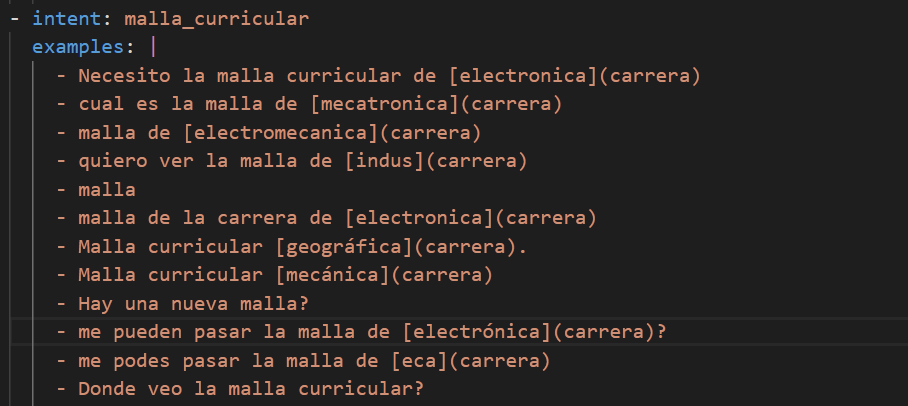
\includegraphics[angle=0,width=0.3\textwidth]{Figuras/Intent-Entities.png}
\par \end{centering}
\caption[Intenciones y Entidades]{Intenciones y Entidades. \textbf{Fuente:} Propia}
\label{Intent_Entities}
\end{figure}
    \item \textbf{slots:} es un registro de datos que Rasa utiliza para guardar la información proveída por el usuario en el curso de la conversación, un claro ejemplo del uso de este elemento es almacenar el nombre del usuario para personalizar los mensajes.
\begin{figure}[H]
\begin{centering}
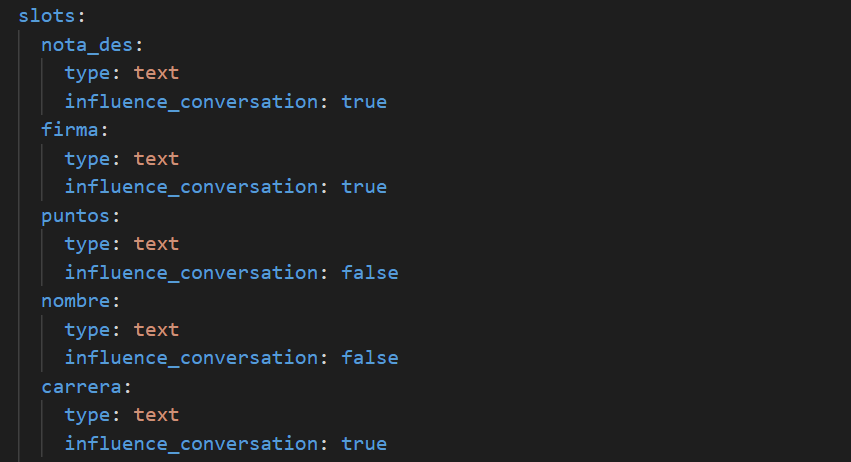
\includegraphics[angle=0,width=0.3\textwidth]{Figuras/Slots.png}
\par \end{centering}
\caption[Slots]{Slots. \textbf{Fuente:} Propia}
\label{Slots}
\end{figure}
    \item \textbf{responses (respuestas):} mensajes que los chatbots envían a los usuarios, estos pueden ser dinámicos y con cualquier tipo de contenido como texto, imágenes, links, etc.
\begin{figure}[H]
\begin{centering}
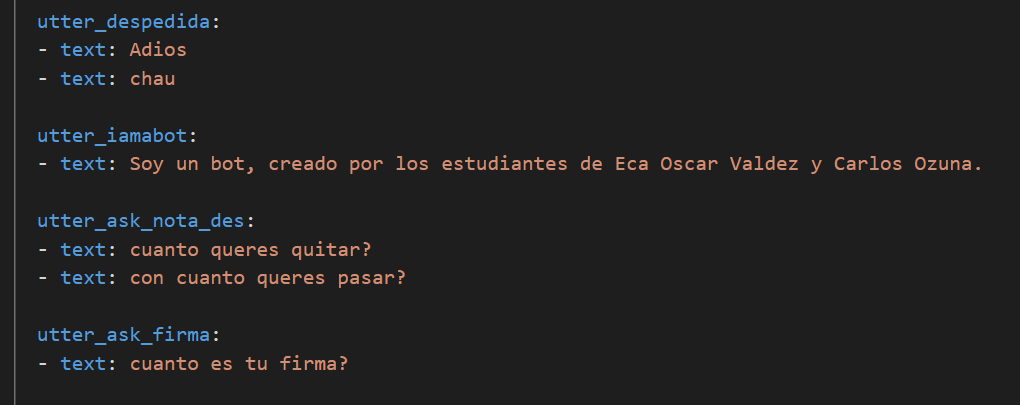
\includegraphics[angle=0,width=0.3\textwidth]{Figuras/Responses.png}
\par \end{centering}
\caption[Respuestas]{Respuestas. \textbf{Fuente:} Propia}
\label{Responses}
\end{figure}
    \item \textbf{forms (formularios):} Un tipo de acción personalizada que pide al usuario varios datos.
\begin{figure}[H]
\begin{centering}
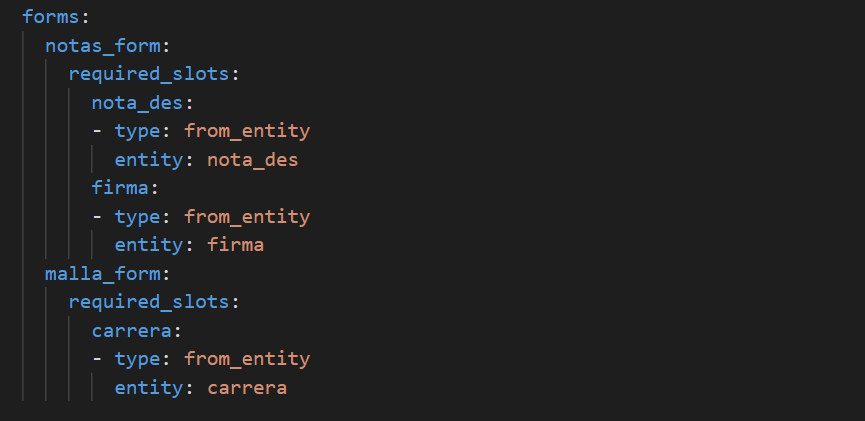
\includegraphics[angle=0,width=0.3\textwidth]{Figuras/Forms.png}
\par \end{centering}
\caption[Acciones]{Acciones. \textbf{Fuente:} Propia}
\label{Acciones}
\end{figure}
    \item \textbf{actions (acciones):} es un paso que toma el bot en la conversación por ejemplo, llamar a una API o enviar una respuesta al usuario.\cite{Glossary}
\begin{figure}[H]
\begin{centering}
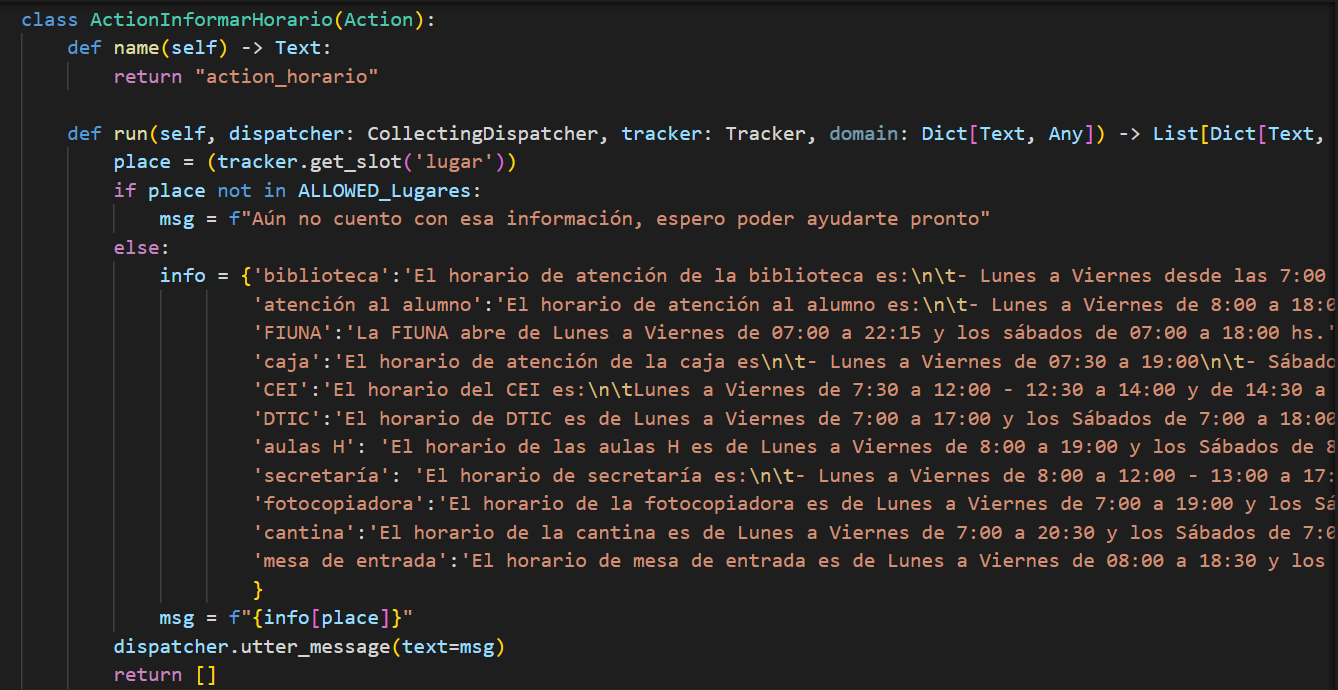
\includegraphics[angle=0,width=0.3\textwidth]{Figuras/actions.png}
\par \end{centering}
\caption[Acciones]{Acciones. \textbf{Fuente:} Propia}
\label{Actions}
\end{figure}
\end{itemize}
\subsection{¿Cómo se llevan a cabo las conversaciones?}
Para llevar a cabo las conversaciones se utilizan las dos librerías del Rasa Stack.
\begin{itemize}
    \item \textbf{Rasa NLU: } En ella  se escriben los archivos de configuración, se elige el pipeline y el modelo de entrenamiento para que deduzca las intenciones y posteriormente pueda extraer las entidades disponibles.\\
    \indent Puede ser basado en reglas o en redes neuronales, el primero suele ser más ligero y no necesita de muchos datos aunque no son buenos en tareas antes no vistas, mientras que el segundo necesita de más capacidad de cómputo y datos para entrenamiento, son más flexibles que los basados en reglas, ya que pueden aprender cosas que no han visto antes.
    \item \textbf{Rasa Core: } es el gestor de diálogos utilizado para crear modelos que sean capaces de decidir que respuestas o acciones se ejecutarán de acuerdo a las entradas generadas por el usuario.\\
    También puede ser basado en reglas, que es el enfoque más tradicional, funciona muy bien en muchos casos pero es difícil de expandir las conversaciones, también puede ser basado en redes neuronales que escoge la siguiente acción basándose en la conversación y en los ejemplos del entrenamiento.
\end{itemize}
\indent Básicamente, Rasa NLU se encarga de interpretar los mensajes y Rasa Core de de decidir que acción tomar.\\
\indent Para asegurarnos de que una conversación funcione se utiliza un proceso denominado ‘conversation-driven development’ que consiste en revisar manualmente las conversaciones para detectar cualquier error cometido, agregar nuevos datos de entrenamiento, volver a entrenar el modelo y probarlo nuevamente. \cite{Introduction_to_Rasa}
\begin{figure}[H]
\begin{centering}
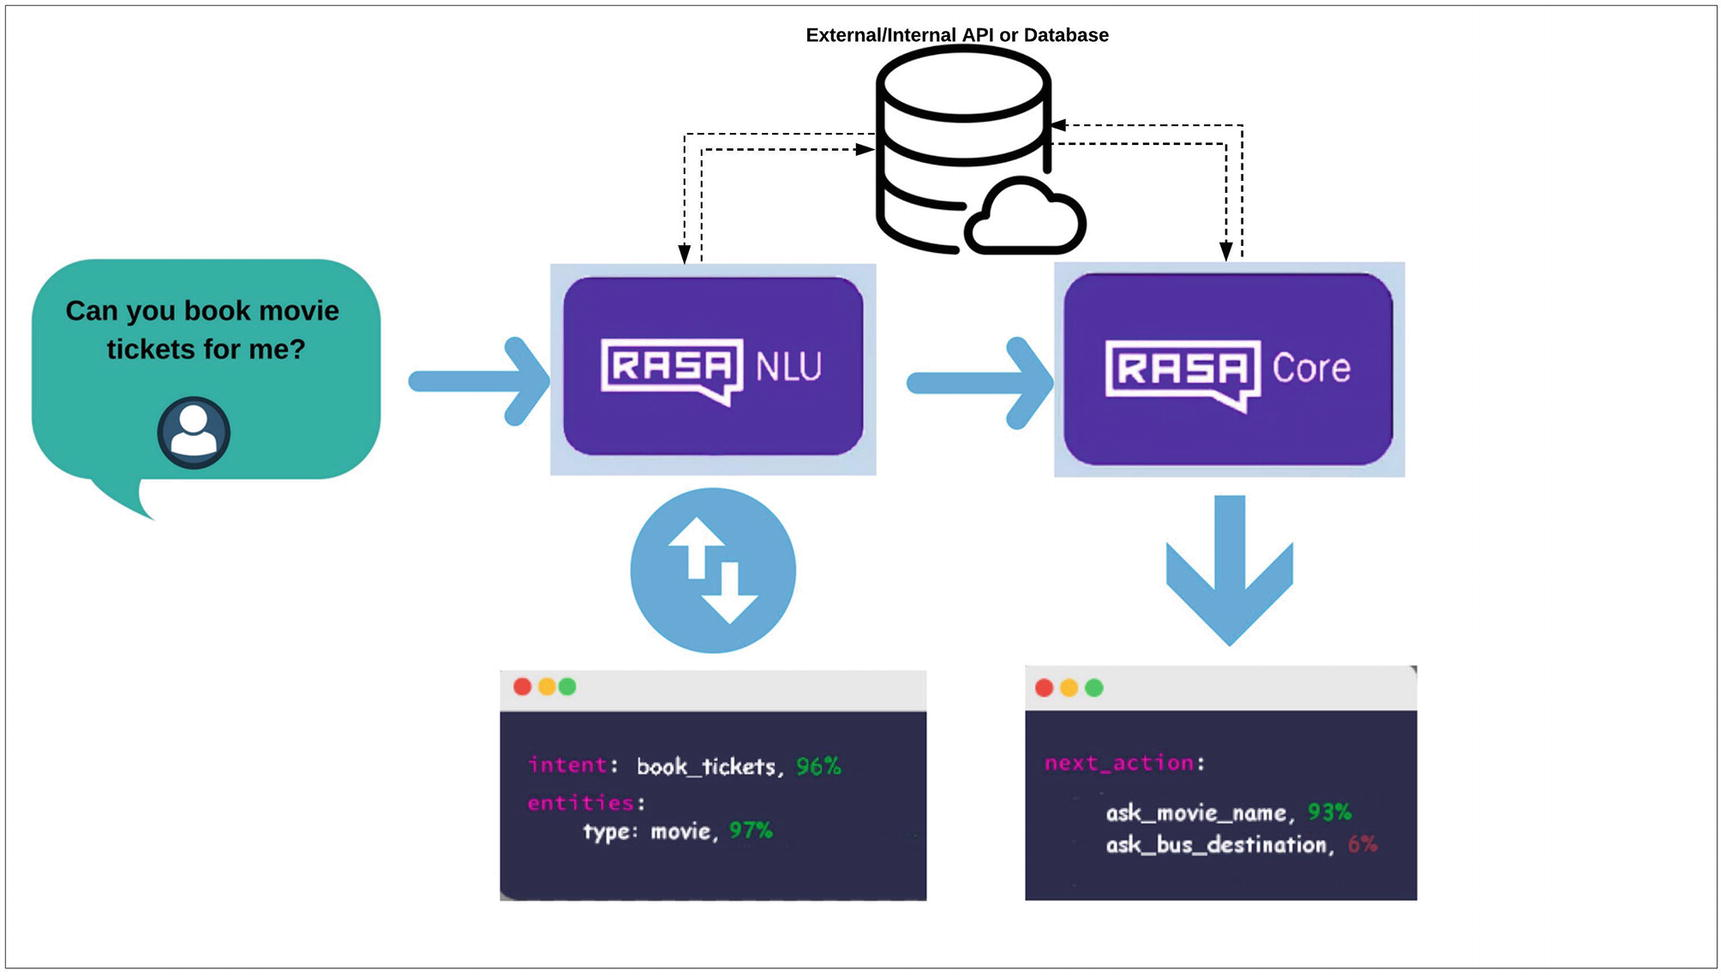
\includegraphics[angle=0,width=0.3\textwidth]{Figuras/NLU-CORE.png}
\par \end{centering}
\caption[Rasa Core y Rasa NLU]{Rasa Core y Rasa NLU. \textbf{Fuente:} \cite{Rasa_Core-NLU}}
\label{Core-NLU}
\end{figure}

\subsection{Creación del Proyecto}
La creación de un nuevo proyecto se realiza con el comando ’rasa init’, éste crea
un conjunto de carpetas y archivos así como se muestra en la siguiente figura.
\begin{figure}[H]
\begin{centering}
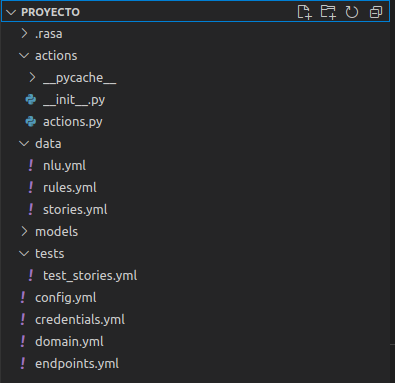
\includegraphics[angle=0,width=0.3\textwidth]{Figuras/4_Estructura del Proyecto.png}
\par \end{centering}
\caption[Estructura del Proyecto]{Estructura del Proyecto. \textbf{Fuente:} Propia}
\label{Estructura}
\end{figure}
\subsubsection{Archivo nlu}
En él se encuentran datos estructurados que sirven para entrenar el modelo y luego extraer la información de los mensajes del usuario. Estos datos son  las intenciones y entidades, también se pueden agregar expresiones regulares y algunas tablas de búsqueda. \cite{NLU_Documentation}
\subsubsection{Archivo Rules}
En este archivo se definen las reglas, que no son más que  tipo de datos de entrenamiento encargados de describir partes de una conversación que siempre sigue el mismo camino.\cite{Rules_Documentation}
\subsubsection{Archivo Stories}
Las historias son un tipo de datos de entrenamiento, se utiliza para entrenar modelos que puedan generalizar las rutas de conversación. Las entradas del usuario son expresadas mediante intents, y entitites si es necesario,  mientras que las respuestas del asistente son expresadas mediante actions.\\
Los patrones que siguen las conversaciones podemos extraer de datos ya existentes o con la herramienta de rasa 'interactive learning'. \cite{Stories_Documentation}
\subsubsection{Archivo config}
En el archivo config se definen el lenguaje y los componentes del pipeline, que forman parte de Rasa NLU y las políticas a ser utilizadas, correspondiente a Rasa NLU.\\
El pipeline es el encargado de definir la dirección de flujo de datos entre los diferentes componentes, Rasa nos permite configurar cada uno de ellos según nuestras necesidades, de tal forma que podamos realizar las predicciones de las intenciones y la extracción de las entidades. Las políticas forman parte de la gestión de diálogos, encargada de seleccionar la siguiente acción a ser ejecutada. \cite{Configuration_Documentation}
La configuración del pipeline y las políticas son de suma importancia, por lo que se detallaran sus componentes en otra sección.
\subsubsection{Archivo credentials}
Aquí se definen los credenciales para las plataformas de voz y chat que el bot utiliza. Rasa cuenta con algunos conectores preestablecidos para los canales más conocidos como Facebook Messenger, Telegram, Google Hangouts Chat o una pagina web propia. \cite{Credentials_Documentation}
\subsubsection{Archivo domain}
El archivo domain es un archivo de configuración donde se especifican las intenciones, entidades, slots, respuestas, formularios y acciones que el bot debe saber. \cite{Domain_Documentation}
\subsubsection{Archivo endpoints}
Los endpoints son los enlaces a los servicios externos o internos que puede tener Rasa. En el se definen los servidores que corren o en los que están alojadas las acciones personalizadas, al igual que los modelos con los que se cuenta. También es aquí donde se especifican los tracker store, utilizados para guardar las conversaciones, y los event broker, encargados de conectar el bot con otros servicios que procesan los datos que llegan de las conversaciones.
\subsection{Componentes}
En esta sección estaremos describiendo el funcionamiento de los componentes
utilizados en la arquitectura de Rasa, estos componentes son modulares y gené-
ricos para lo que son sistemas de NLU modernos, pueden ser propios del entorno
o proveídos por otras librerías de terceros para extender funcionalidades
\begin{figure}[H]
\begin{centering}

\includegraphics[angle=0,width=0.3\textwidth]{Figuras/Componentes_NLU.png}
\par \end{centering}
\caption[Componentes del NLU]{Componentes del NLU. \textbf{Fuente:} Propia}
\label{Estructura}
\end{figure}
\subsubsection{Tokenizadores}
Antes de poder ser procesada una porción de texto debe ser dividida en porciones más pequeñas, para esto se utiliza 
un tokenizador (o tokenizer).   Este divide el texto en componentes de un vector.
\subsubsection{Caracterizadores}
Los caracterizadores generan pesos numéricos para ser consumidos por los modelos de ML. Existen dos tipos principales de
características, las Dispersas (Sparse Features) que pueden representar subpalabras o características
léxicas, estas son las utilizadas para que aprendan los significados del dominio, y las Densas (Dense Features) que suelen consistir en porciones preentrenadas, útiles especialmente al iniciar un proyecto y no se cuenta con suficientes datos de entrenamiento.
\begin{table}[h]
\resizebox{0.49\textwidth}{!}{%
\begin{tabular}{|l|l|l|}
\hline
\textbf{Caracterizador}    & \textbf{Requisitos}     & \textbf{Tipo}                                                                  \\ \hline
MitieFeaturizer            & MitieNLP                & Dense featurizer                                                               \\ \hline
SpacyFeaturizer            & Dense / Sparse Features & \begin{tabular}[c]{@{}l@{}}Logistic Regression de \\ scikit-learn\end{tabular} \\ \hline
ConveRTFeaturizer          & Tokenization            & Dense featurizer                                                               \\ \hline
LanguageModelFeaturizer    & Tokenization            & Dense featurizer                                                               \\ \hline
CountVectorsFeaturizer     & Tokenization            & Sparse featurizer                                                              \\ \hline
LexicalSyntactitFeaturizer & Tokenization            & Sparse featurizer                                                              \\ \hline
RegexFeaturizer            & Tokenization            & Sparse featurizer                                                              \\ \hline
\end{tabular}%
}
    \caption{ Caracterizadores. Elaboración Propia}
    \label{tab:Caracterizadores}
\end{table}
\subsubsection{Extractor de Entidades}
Los extractores de entidades son herramientas que se utilizan para identificar y extraer información relevante de un texto, como son los nombres, lugares o números. Dependiendo de la situación, puede ser implementado un extractor basado en Expresiones
Regulares o extractores basados en Aprendizaje Automático.
\begin{table}[h]
\resizebox{0.49\textwidth}{!}{%
\begin{tabular}{|l|l|l|}
\hline
\textbf{Clasificador}   & \textbf{Requisitos} & \textbf{Utiliza}                                                            \\ \hline
MitieEntityExtractor    & MitieNLP            & \begin{tabular}[c]{@{}l@{}}Clasificación multiclase \\ con SVM\end{tabular} \\ \hline
SpacyEntityExtractor    & SpacyNLP            & Modelo estadístico BILOU                                                    \\ \hline
CRFEntityExtractor      & Tokens              & Campo aleatorio condicional (CRF)                                           \\ \hline
DucklingEntityExtractor & Ninguno             & Expresiones regulares                                                       \\ \hline
DIETClassifier          & Dense Features      & Transformadores                                                             \\ \hline
RegexEntityExtractor    & Ninguno             & Tablas de búsqueda                                                          \\ \hline
\end{tabular}%
}
\caption{Extractores de entidades. Elaboración propia}
\label{EntityExtractor}
\end{table}
\subsubsection{Clasificador de Intenciones}
Una vez que se generaron las características para todos los tokens y para toda la oración, podemos pasarlos a un
modelo clasificador de intenciones para obtener la intencion detrás de cada mensaje de usuario y posteriormente poder brindarle una respuesta adecuada.
\begin{table}[h]
\resizebox{0.49\textwidth}{!}{%
\begin{tabular}{|l|l|l|}
\hline
\textbf{Clasificador}        & \textbf{Requisitos}     & \textbf{Utiliza}                                                                              \\ \hline
MitieIntentClassifier        & MitieNLP                & Clasificación multiclase con SVM                                                              \\ \hline
LogisticRegressionClassifier & Dense / Sparse Features & Logistic Regression de scikit-learn                                                           \\ \hline
SklearnIntentClassifier      & Dense Features          & \begin{tabular}[c]{@{}l@{}}SVM lineal optimizado con búsqueda \\ en cuadrícula\end{tabular}   \\ \hline
KeywordIntentClassifier      & Ninguno                 & Comparador de palabras clave                                                                  \\ \hline
DIETClassifier               & Dense Features          & Transformadores                                                                               \\ \hline
FallbackClassifier           & Intents                 & \begin{tabular}[c]{@{}l@{}}Requiere de un clasificador de \\ intenciones previo\end{tabular} \\ \hline
\end{tabular}%
}

\caption{Clasificadores de intenciones. Elaboracion propia}
\label{IntentClassifier}
\end{table}
 \subsection{Predicción de Acciones}
Con el flujo NLU, se detectan las entidades e intenciones. Pero este flujo no predice la siguiente acción en la 
conversación. Para esto se utiliza el flujo de política. Las políticas aseguran el uso de predicciones de NLU así como 
también el estado presente de la conversaciones para decidir que acción tomar, pueden ser basado en reglas o en aprendizaje automático.
\textbf{Políticas basadas en Aprendizaje Automático:}
\begin{itemize}
    \item \textbf{TED Policy:}
    Es un conjunto de algoritmos desarrollados por RASA para la predicción de diálogo y reconocimiento de entidades. Su arquitectura se basa en transformadores que convierten el diálogo actual en un vector de diálogos, para compararlos con otros vectores en busca del más cercano, a partir de las acciones existentes.\cite{TED_Policy}
    \item \textbf{UnexpecTED Intent Policy:} Es una política auxiliar, tiene la misma arquitectura que TEDPolicy pero éste aprende cuales son las intenciones más probables a ser expresadas según el contexto de la conversación. Siempre debe usarse en conjunto con al menos una otra política.\cite{UnexpecTED}
    \item \textbf{Memoization Policy: }Esta política utiliza las historias y acciones de los datos de entrenamiento y las guarda en un diccionario, si la conversación actual no coincide con ningun ejemplo, predice un 0.0, se aplica cuando la los datos ingresados son similares a un historia existente.\cite{MemoizationPolicy}
    \item \textbf{Augmented Memoization Policy: } Tiene las mismas funcionalidades de Memoization Policy, pero además cuenta con un mecanismo que permite olvidar de forma aleatoria algunas partes de la conversación, luego predice las acciones ya con la historia reducida.\cite{AugmentedMemoizationPolicy}
\end{itemize}
\textbf{Políticas basadas en Reglas:}
\begin{itemize}
    \item \textbf{Rule Policy:} Realiza las predicciones basandose en reglas que se tienen en los datos de entramiento.
\end{itemize}
\indent Con cada interacción, las políticas definidas indican con un nivel de confianza cuál será la siguiente acción a ser tomada, aquella que tiene obtiene el mayor resultado será la que decida la siguiente acción, en caso de que se prediga con la misma confianza, se tiene en cuenta la siguiente asignación de importancia.
\begin{itemize}
    \item 6 - RulePolicy
    \item 3 - MemoizationPolicy o AugmentedMemoizationPolicy
    \item 2 -  UnexpecTEDIntentPolicy
    \item 1 - TEDPolicy
\end{itemize}
%oscar-ozuna

\section{Implementación}
En la siguiente sección se presentan los componentes elegidos y sus funciones en el
sistema.
\subsection{Configuración del Pipeline}
\begin{itemize}
	\item \textbf{WhitespaceTokenizer}: componente que divide el texto en palabras
	      individuales, utilizando espacios en blanco como delimitador.
	      \cite{Configuration_Documentation}
	\item \textbf{RegexFeaturizer}: componente que crea características basadas en expresiones
	      regulares. Esto puede ser útil para detectar patrones en el texto.
	      \cite{Configuration_Documentation}
	\item \textbf{LexicalSyntacticFeaturizer}: componente que combina características léxicas y
	      sintácticas para crear una mejor representación del texto. Utiliza etiquetas de
	      partes del discurso
	      y etiquetas de análisis de dependencia para crear características.
	      \cite{Configuration_Documentation}
	\item \textbf{CountVectorsFeaturizer}: componente que crea una representación dispersa de
	      bolsa de
	      palabras del texto. Puede ser utilizado para crear características para la
	      clasificación de
	      intenciones o la extracción de entidades. \cite{Configuration_Documentation}
	\item \textbf{DIETClassifier}: componente que combina una red neuronal recurrente con un
	      transformador para realizar la clasificación de intenciones y el reconocimiento de
	      entidades.
	      Utiliza múltiples fuentes de información, como incrustaciones de palabras,
	      incrustaciones de
	      caracteres y etiquetas de partes del discurso. \cite{Configuration_Documentation}
	\item \textbf{EntitySynonymMapper}: componente que mapea las entidades a su forma canónica.
	      Esto puede ser útil para manejar variaciones en la forma en que se expresan las entidades o como se
	      conocen en RASA 'sinónimos'\cite{Configuration_Documentation}
	\item \textbf{ResponseSelector}: componente que selecciona una respuesta basada en la
	      entrada del
	      usuario. Utiliza un enfoque basado en recuperación, donde coincide la entrada del
	      usuario con un
	      conjunto de respuestas predefinidas. Puede ser útil para manejar preguntas frecuentes
	      o
	      conversaciones informales.\cite{Configuration_Documentation}
	\item \textbf{FallbackClassifier}: componente que clasifica los mensajes como fallback si
	      no coinciden con ninguna de las intenciones en el modelo. Puede ser útil para manejar mensajes
	      fuera de contexto o solicitudes que el modelo no está entrenado para
	      manejar.\cite{Configuration_Documentation}
\end{itemize}
\subsection{Docker}

Existen varias implementaciones de contenedores para servidores como Docker, containerd, OpenVZ y
HyperV. La mas utilizada en la industria y con mas variedad de servicios actualmente es
Docker por lo que decidimos elegir esta herramienta para el desarrollo y despliegue de servicios del
proyecto. Docker puede ser ejecutado sobre sistemas basados en Windows, Linux y macOS lo que
facilita la igualdad de condiciones entre ambientes de desarrollo y producción, ademas es de uso
libre y gratuito. \cite{alternativas_docker}

\subsection{Contenedor}

Los contenedores son la unidad más pequeña un sistema, es una entidad que se utiliza para aislar
cada componente del sistema base. Cada contenedor puede aislarse mediante funciones del sistema
operativo llamadas cgroups y cnames logrando así aplicaciones en entornos aislados (sandbox en
Ingles). \cite{Docker}
\begin{figure}[H]
	\begin{centering}
		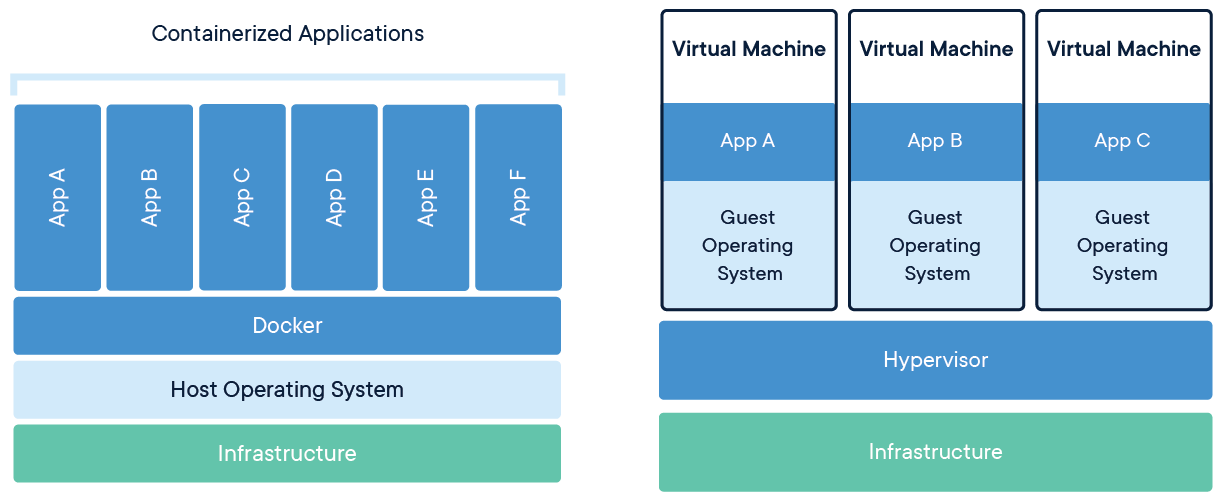
\includegraphics[angle=0,width=0.3\textwidth]{Figuras/docker-container.png}
		\par \end{centering}
	\caption[Contenedores]{Contenedores. \textbf{Fuente:} \cite{Docker}}
	\label{Contenedores}
\end{figure}

\subsection{Imagen de contenedor}
Una imagen de contenedor es el sistema de archivos aislados de todos los archivos necesarios para
ejecutar la aplicación, así como dependencias, configuraciones, ejecutables, etc. Así como también
variables de entorno y datos necesarios para ejecutar la aplicación. \cite{Docker}

\subsection{Redes}
Entre las ventajas de desplegar una aplicación por medio de contenedores Docker es que se pueden
comunicar entre ellos y también con servicios externos al entorno de Docker. Por defecto se pueden
crear varios tipos de configuraciones de red, pero por lo general se utilizan redes puente entre
los contenedores para que estos puedan comunicarse mutuamente entre ellos y solo exponiendo los
puertos necesarios para interactuar con el sistema en cuestión y esta es la opción utilizada en
nuestra implementación. \cite{Docker}

\subsection{Volúmenes}
Puesto que un contenedor no tiene un estado persistente sobre los datos que genera, se introducen
los volúmenes, son la forma recomendada de agregar persistencia de datos a un contendedor de
Docker. \cite{Docker}
\begin{figure}[H]
	\begin{centering}
		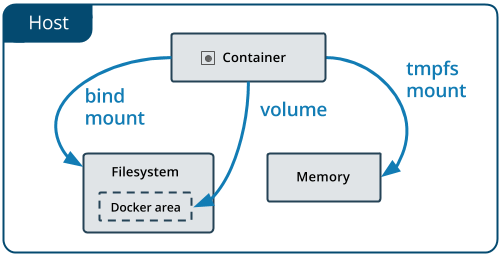
\includegraphics[angle=0,width=0.3\textwidth]{Figuras/docker-volume.png}
		\par \end{centering}
	\caption[Volumen]{Volumen. \textbf{Fuente:} \cite{Docker}}
	\label{Volumen}
\end{figure}

\subsection{Construcción}
Las imágenes de Docker se construyen partir de instrucciones escritas en un archivo denominada
Dockerfile, generalmente de parte de una imagen base de la cual sé la adiciona lo necesario para
ejecutar la aplicación.
\cite{Docker}

\subsection{Repositorios}
Un repositorio de imágenes Docker (Docker Registry) es un servidor que almacena y distribuye
imágenes versionadas generadas partir de un Dockerfile. Estos repositorios pueden ser públicos como
DockerHub que es el oficial de la comunidad de Docker, como así también privado para un equipo de
desarrollo en una institución. \cite{Docker}

\subsection{Componentes}
Cada componente del sistema se configuró en un contenedor de Docker con la excepción del servidor
NGINX que si estaba instalado sobre el sistema operativo del servidor.
\begin{figure}[H]
	\begin{centering}
		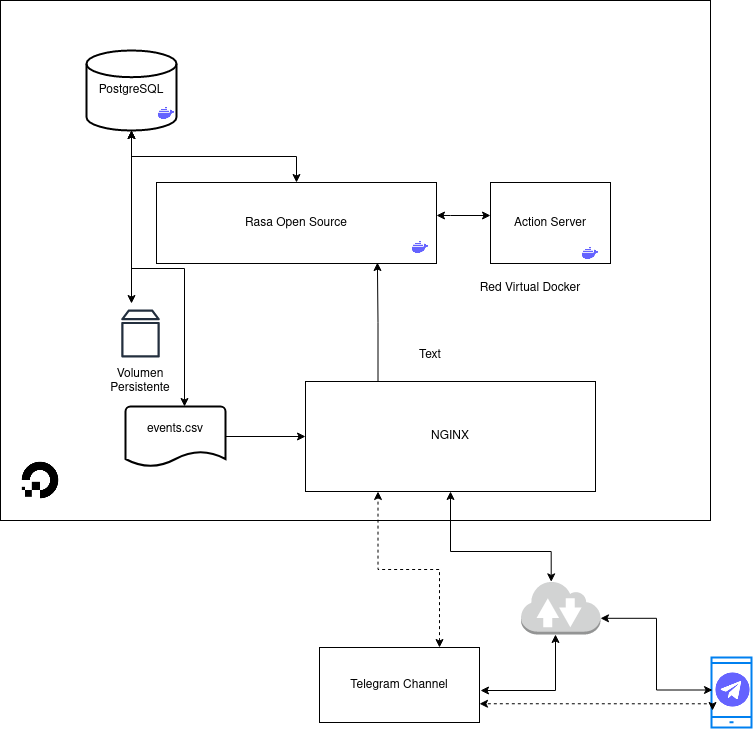
\includegraphics[angle=0,width=0.3\textwidth]{Figuras/server.png}
		\par \end{centering}
	\caption[Componentes del Sistema]{Componentes del Sistema. \textbf{Fuente:} Elaboración propia.}
	\label{Componentes}
\end{figure}
\subsection{Rasa Open Source}
El contendedor de Rasa Open Source ejecuta una imagen oficial proveída por Rasa disponible en los
repositorios de DockerHub \cite{DockerHub}, pero con el modelo entrenado y las configuraciones
particulares al proyecto. Es el único contenedor que tiene un puerto externo para servir al
usuario. También hace uso de los servicios de PosgresSQL y del servicio de acciones (action
server).

\subsection{Servidor de acciones}
Servidor de acciones (action server) es un servicio interno que ejecuta código escrito en Python
este utiliza una imagen oficial para servicios Python disponible en los repositorios de
DockerHub \cite{DockerHub}, estas son operaciones específicas para algunas acciones, una respuesta
no estática, como por el ejemplo la acción relacionada con el cálculo de puntajes en el final de
acuerdo a los puntajes en los exámenes parciales.

\subsection{PostgresSQL}
En la documentación de Rasa, especifica que se necesita un almacenamiento para el registro de
eventos (event broker) para su posterior análisis o también para el procesamiento de los eventos
por otros
servicios. Dependiendo de la demanda y el flujo de datos se pueden elegir Pika, Kafka y asi como
el uso de Bases de datos basadas en SQL para el almacenamiento. \cite{event_broker} Como
contábamos con experiencia previa en el uso de bases de datos utilizamos PostgresSQL que era una
implementación ya conocida, ademas para el desarrollo las funcionalidades adicionales de  si bien
podrían haber sido útiles agregarían complejidad innecesaria al sistema en fases iniciales y pueden
ser adicionados posteriormente.
PostgresSQL es un motor de base de datos del tipo relacional\cite{postgresql} el cual se configuró
a partir de una imagen oficial de PostgresSQL disponible en los repositorios de
DockerHub\cite{DockerHub}. Aparte de sus funciones de base de datos de sistema, también ejecutar un
trabajo periódico(cada una hora) para realizar una copia actualizada de los contenidos de la tabla
Eventos a un archivo separado por comas(csv) que se utiliza para retroalimentar las conversaciones
y generar más datos para mejorar el modelo.

\subsection{NGINX}
Para poder servir los archivos y la redirección interna de  las peticiones al servidor de Rasa Open
Source se necesita un servidor WEB con estas características. Existen  varias implementaciones que
pueden ser útiles como Apache, Caddy y NGINX. El mas utilizado en la industria es NGINX por lo que
elegimos por su facilidad para configuración, amplia disponibilidad de documentación y asi como
también ser el mas eficiente entre las demás opciones. \cite{web_servers}
NGINX, es un servidor web que también puede ser usado como proxy reverso, que implica redirigir el
tráfico a puertos internos y también para servir archivos que fueron las funciones utilizadas para
el proyecto. Así como también puede ser utilizado como balanceador de carga, mail proxy y HTTP
cache, entre otras funciones \cite{NGINX}
El servidor NGINX redirige el tráfico a la instancia de Rasa Open Source y si como también sirve el
archivo de
la copia más reciente de la tabla Eventos para agilizar las verificaciones de las respuestas y
preguntas recibidas.
\subsection{Recursos}
Para la puesta en producción del proyecto, se utilizó una instancia de Droplet alojado en Nueva
York del proveedor DigitalOcean con un procesador con un 1vcpu(procesador virtualizado), 1 GB de
RAM, 25 GB de almacenamiento y con un costo de entre 4 y 6 dólares americanos al mes dependiendo
del tráfico presentado. Por las limitaciones de memoria del servidor se configuró también 4 GB de
espacio de intercambio(SWAP) en el espacio de almacenamiento.


\subsection{Telegram}
Entre las opciones de interfaz existen dos opciones populares, implementar un cliente web o
aplicación Movil, o integrarlo dentro de plataformas de mensajería existentes. Para evitar agregar
complejidad al sistema decidimos optar por el uso de una plataforma existente. Si bien la plataforma
de mensajería mas utilizada en nuestro medio es WhatsApp, esta presenta
costos para el uso de su interfaz de programación por lo que fue descartada para la implementación del
proyecto, la segunda mas utilizada es Telegram que debido a su una amplia comunidad
para desarrollo de soluciones dentro de la plataforma puesto que es bastante sencillo
usar su servicio para conectar a implementaciones de chatbots, ademas no requiere costos para el
uso de su interfaz de programación por lo que consideramos que era la mejor opción para
publicar la solución a los usuarios finales.
\cite{botfather}

\section{Resultados}
Inicialmente, se creó un conjunto de datos con las posibles preguntas frecuentes de los alumnos,
una vez que el Bot estuvo en funcionamiento e integrado a Telegram se recolectaron las preguntas
que realmente tienen los estudiantes de la FIUNA, estas fueron guardadas en una base de datos como
eventos, teniendo mucha información innecesaria para el conjunto de datos. Para un mejor manejo y
limpieza de los datos se utilizó Python con ayuda de la librería Pandas. Posteriormente se guardó
el dataframe creado en un archivo de Excel donde se analizaron y clasificaron un total de 1051
entradas en 141 intenciones distintas, De entre ellas, se identificaron las 15 intenciones más
recurrentes.

\begin{figure}[H]
	\centering
	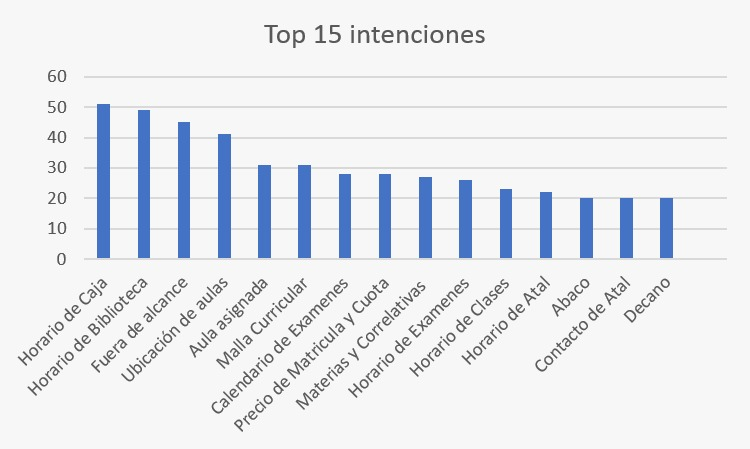
\includegraphics[angle=0,width=0.3\textwidth]{Figuras/Top15intents.jpeg}
	\caption{Top 15 Intenciones}
	\label{fig:Top15intents}
\end{figure}

\subsection{Validación de los datos e Historias}
Rasa cuenta con varias funciones para probar los diálogos, historias, gestor de diálogos y el
procesamiento de mensajes, de tal forma a encontrar errores o inconsistencias antes de realizar el
entrenamiento.

\subsubsection{Validación de datos}
El siguiente comando se encarga de verificar que no haya errores e inconsistencias en los datos y
configuraciones.

\begin{center}
	\framebox[5cm][c]{rasa data validate}
\end{center}

Es recomendable ejecutarlo antes de entrenar el modelo, ya que si se encuentra algún problema, el
entrenamiento también podría fallar.

\subsection{Evaluación del desempeño de la NLU}
Una práctica usual al ejecutar aprendizaje automático es dividir aleatoriamente el conjunto de
datos en uno de entrenamiento y otro de pruebas. El bot utiliza el primer conjunto para aprender
las características necesarias para realizar las predicciones adecuadas, y el segundo conjunto para
evaluar el modelo mediante datos que aún no hayan sido vistos antes.\\
Rasa nos permite dividir los datos mediante el comando:

\begin{center}
	\framebox[5cm][c]{rasa data split nlu}
\end{center}

Por defecto, Rasa separa los datos de entrenamiento/prueba en un 80/20, luego, para probar que tan
bien entrenado se encuentra el modelo utilizamos 'rasa test nlu' especificando cuales son los datos
de entrenamiento y prueba de la siguiente forma:\\

\begin{center}
	\framebox[7cm][c]{    --nlu train\_test\_split/test\_data.yml}
\end{center}

Rasa test proporciona herramientas que facilitan la detección y corrección de errores, incluye una
matriz de confusión, un archivo .json de reporte, un histograma de confianza y un archivo .json de
errores en caso de que existan.\\
\indent La matriz de confusión es una herramienta fundamental que permite evaluar el rendimiento de
un
modelo, permite identificar los falsos positivos y falsos negativos, nos muestra en su eje vertical
las etiquetas reales y en el eje horizontal las etiquetas predecidas, permitiendo identificar si
existen errores de clasificación.\\
\indent Además, el script de rasa test guarda estos errores de clasificación en un archivo .json lo
que
facilita el depurado y corrección de errores para mejorar la calidad de la clasificación.\\
\indent El Histograma nos permite visualizar las predicciones del modelo y la confianza que ha sido
otorgada a cada intención o entidad.\\
\indent Las predicciones correctas se encuentran en la parte izquierda del gráfico y son
representadas en
color azul, mientras que las incorrectas se encuentran a la derecha y son de color rojo.\\
\indent La ubicación de cada predicción en el eje horizontal del histograma representa el número de
muestras, y en el eje vertical la confianza con la que el modelo ha realizado su predicción.
\cite{interpretacion_graficos}

\subsubsection{Clasificador de Intenciones}
Al analizar la matriz de confusión \ref{fig:intent_matriz} y el histograma
\ref{fig:intent_histograma} podemos verificar que todas las intenciones fueron clasificadas
correctamente con una confianza superior a 0.98, indicando que el modelo es bastante efectivo en su
tarea de clasificación.
\begin{figure}[H]
	\centering
	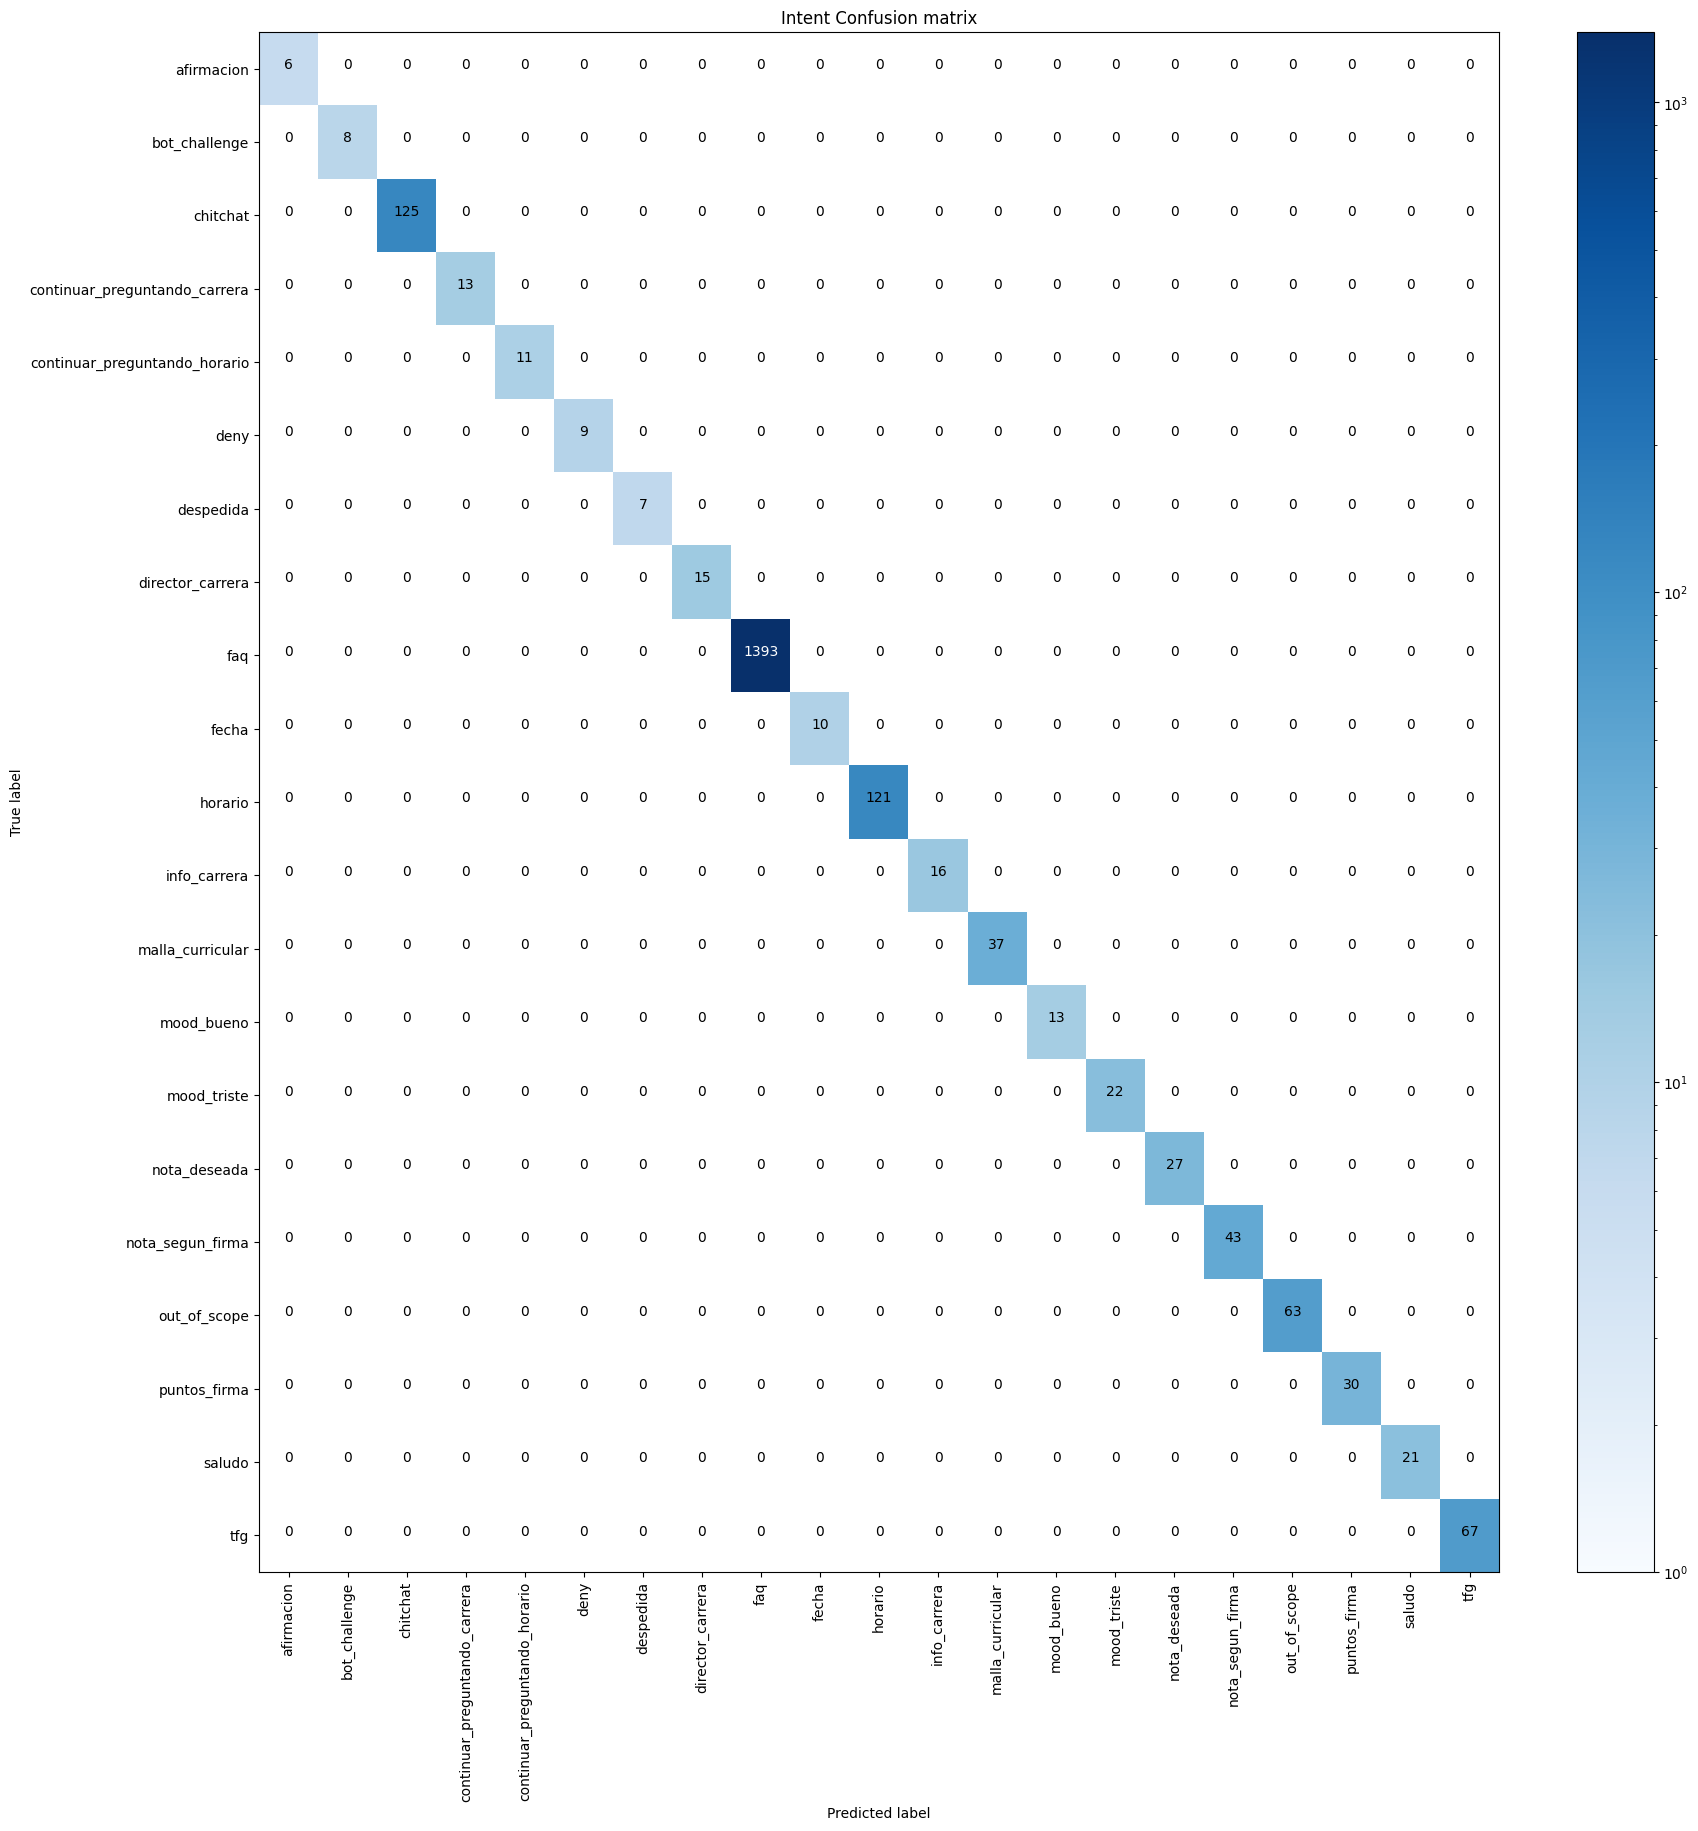
\includegraphics[angle=0,width=0.3\textwidth]{Figuras/intent_confusion_matrix.png}
	\caption{Matriz de Confusión de Intenciones}
	\label{fig:intent_matriz}
\end{figure}

\begin{figure}[H]
	\centering
	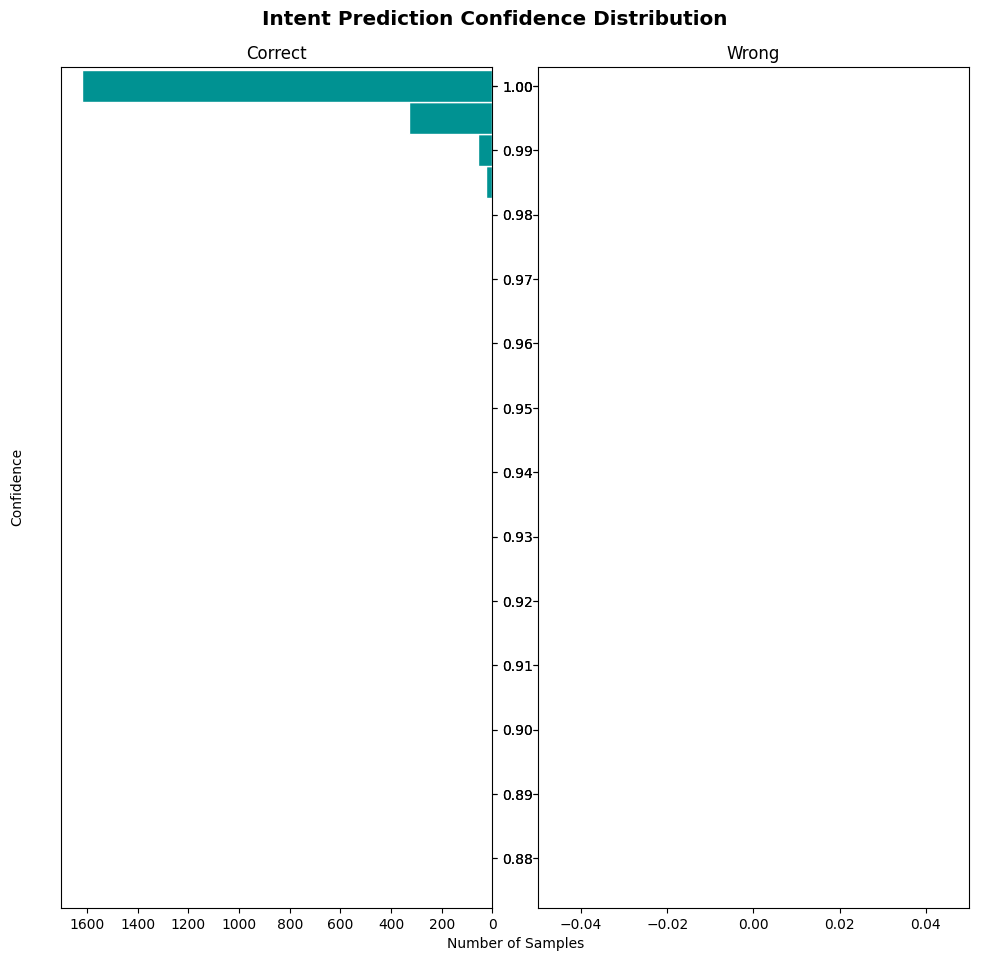
\includegraphics[angle=0,width=0.3\textwidth]{Figuras/intent_histogram.png}
	\caption{Histograma de confianza en la clasificación de Intenciones}
	\label{fig:intent_histograma}
\end{figure}
\subsubsection{Extracción de entidades}
Al ver los gráficos del extractor, tanto en la matriz de confusión de entidades
\ref{fig:entity_matriz} como en el histograma \ref{fig:entity_histograma} se encuentra que el
modelo se confunde con dos entidades, revisando el reporte de errores se encuentra que los
extractores DIETClassifier y EntitySynonymMapper reconocen las entidades por separado, esto genera
el error pero no afecta al rendimiento del modelo o a la correcta selección de una respuesta.

\begin{figure}[H]
	\centering
	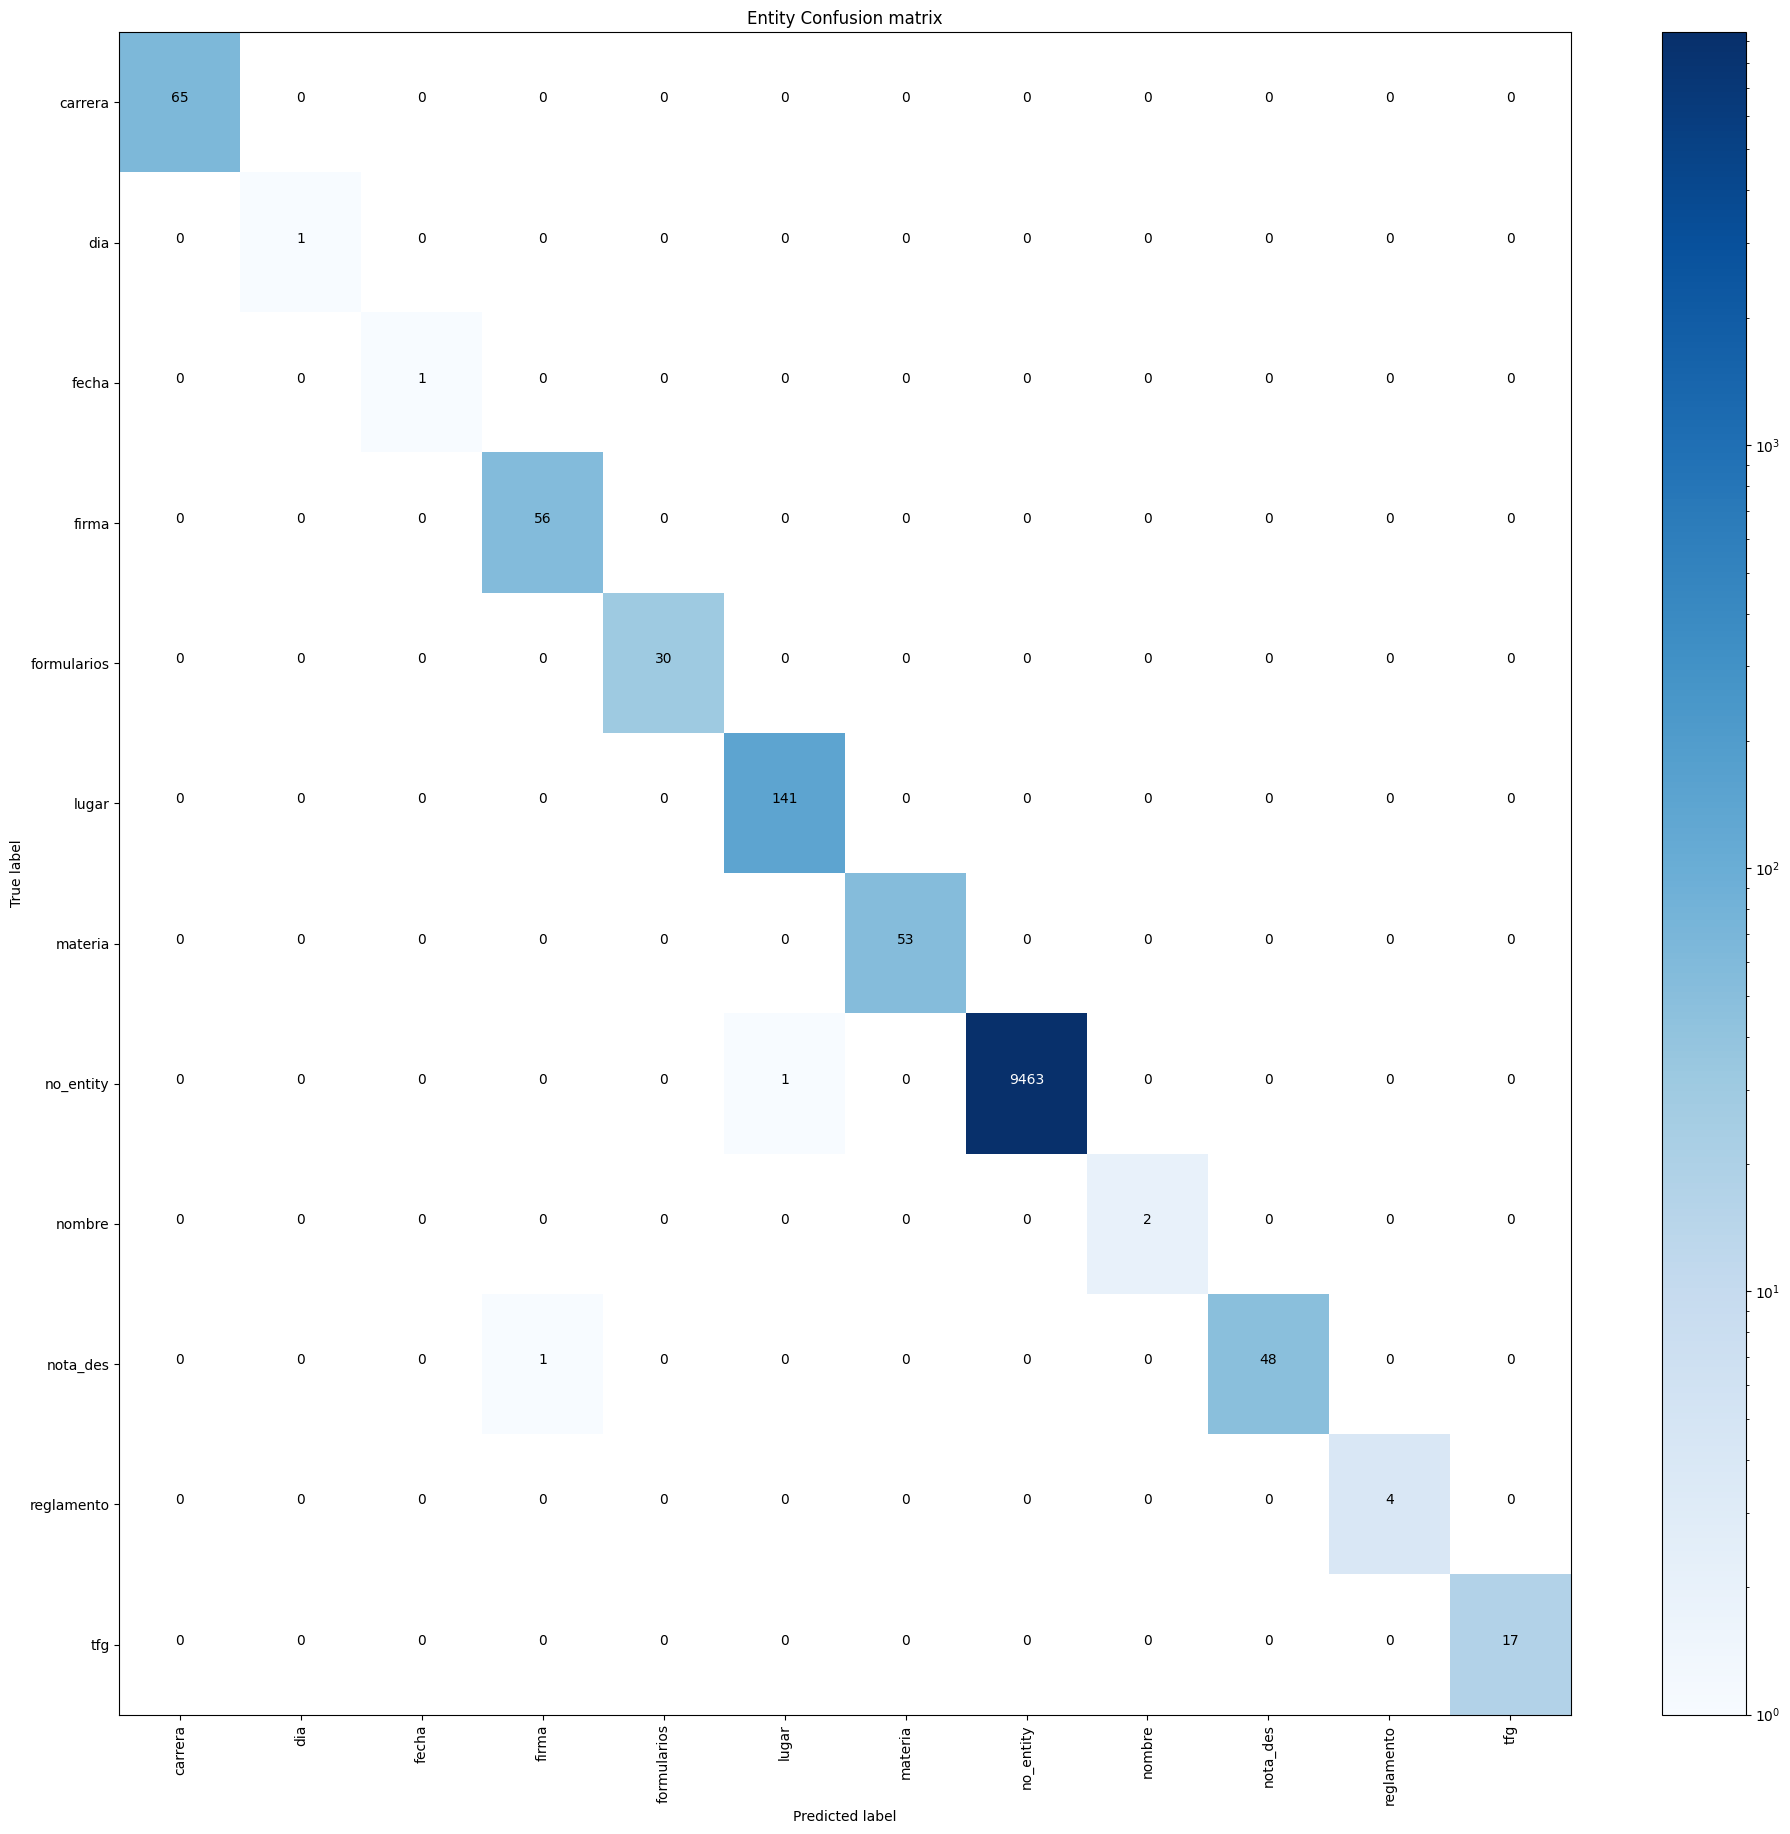
\includegraphics[angle=0,width=0.3\textwidth]{Figuras/DIETClassifier_confusion_matrix.png}
	\caption{Matriz de Confusión del extractor de entidades}
	\label{fig:entity_matriz}
\end{figure}

\begin{figure}[H]
	\centering
	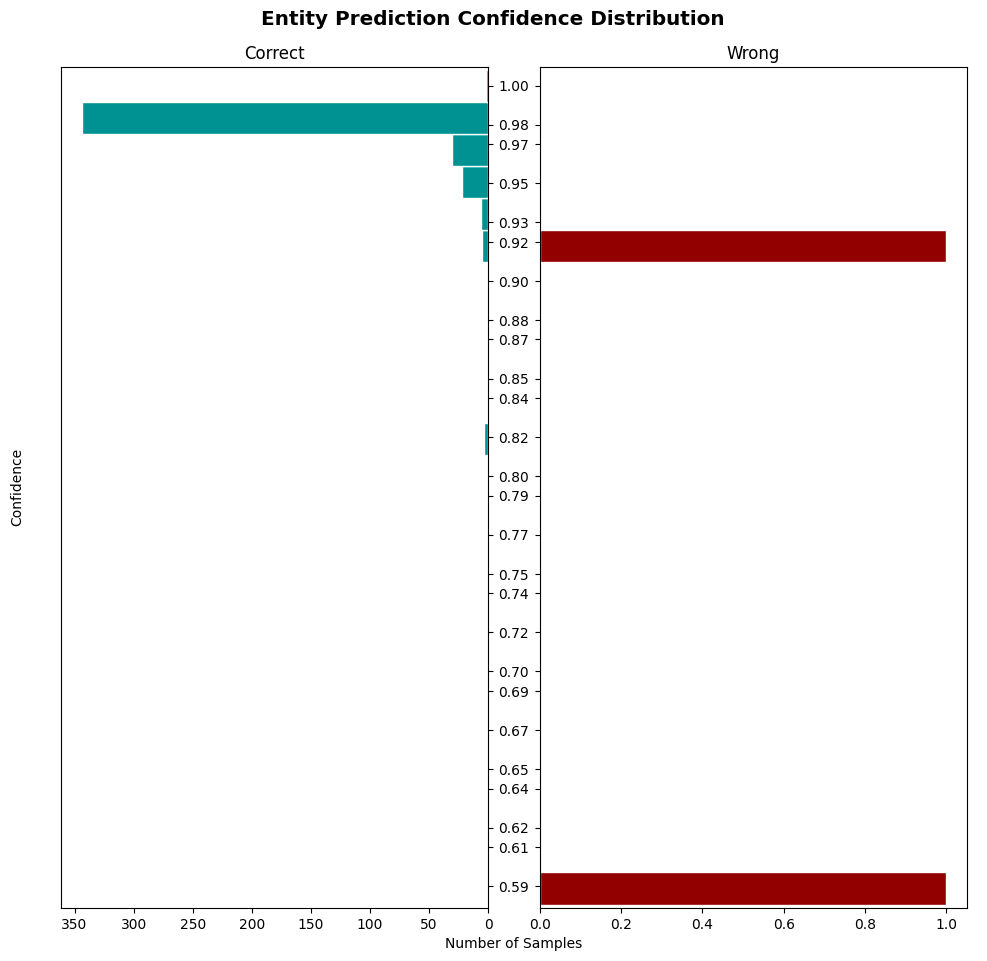
\includegraphics[angle=0,width=0.3\textwidth]{Figuras/DIETClassifier_histogram.png}
	\caption{Histograma de confianza del extractor de entidades}
	\label{fig:entity_histograma}
\end{figure}

\subsubsection{Selección de Respuestas}
Podemos observar en el histograma \ref{fig:response_histograma} de la selección de respuestas que
no se predijo erróneamente ninguna respuesta, la matriz de confusión en este caso no es de mucha
utilidad ya que son bastantes respuestas y complica la visibilidad de las etiquetas, en caso de que
existiese un error podremos encontrarlo en el reporte .json.

\begin{figure}[H]
	\centering
	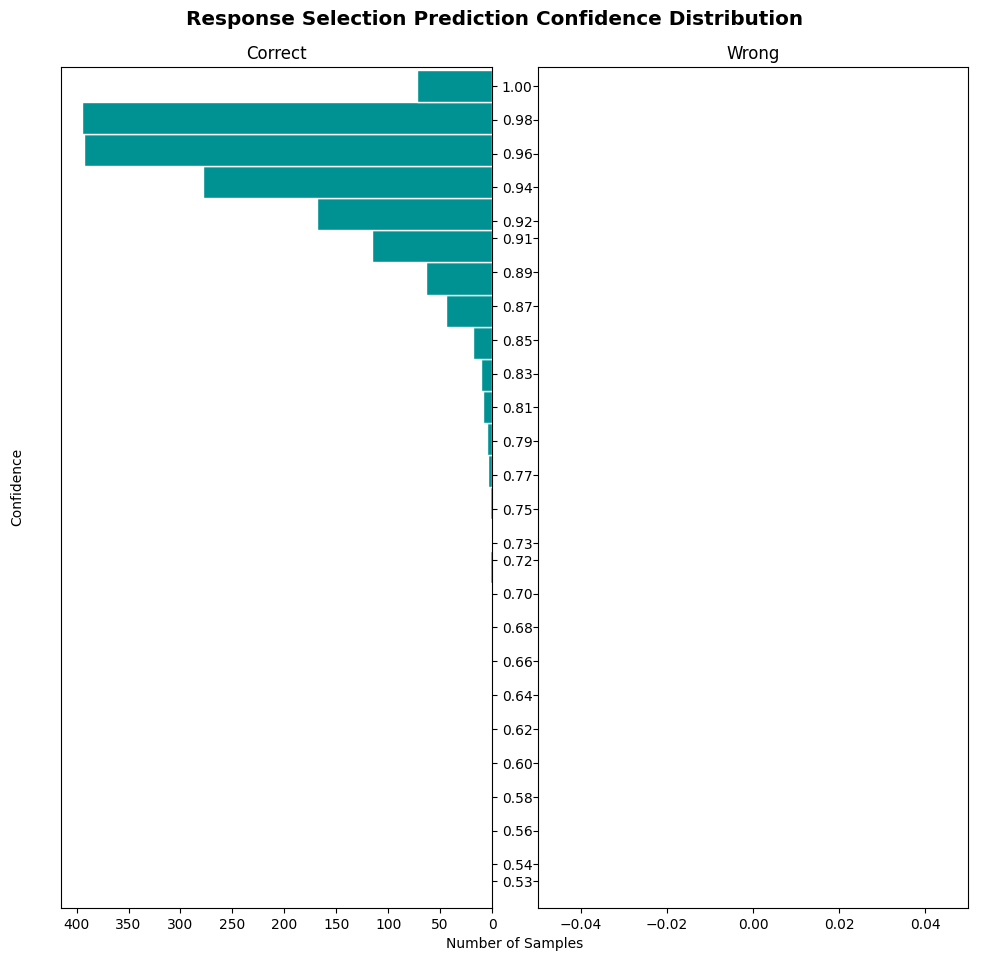
\includegraphics[angle=0,width=0.3\textwidth]{Figuras/response_selection_histogram.png}
	\caption{Histograma de confianza del seleccionador de respuestas}
	\label{fig:response_histograma}
\end{figure}
\section{Posibles Mejoras}
\begin{itemize}
	\item Integrar a sistemas existentes de la Facultad de Ingeniería.
	\item Se puede agregar respuestas de la chatbots públicos como	ChatGPT \cite{api_chatgpt}
	      para preguntas
	      fuera del
	      contexto de la Facultad de Ingeniería.
\end{itemize}%oscar

\section[Conclusiones]{Conclusiones}
\begin{itemize}
	\item Revisamos las tecnologías y plataformas disponibles actualmente para el desarrollo de
	      chatbots institucionales.
	\item Se implementó un chatbot utilizando la plataforma Rasa OpenSource, el cual responde preguntas
	      frecuentes de los estudiantes de la Facultad de Ingeniería.
	\item Se utilizó un dataset inicial propio y se recopilaron preguntas de los alumnos en grupos de
	      prueba para entrenar el modelo.
	\item Seleccionamos, entrenamos y probamos el algoritmo utilizando el dataset generado.
	\item Se implementó un servidor público que alberga los servicios del chatbot.
	\item Se utilizó la API de Telegram para que el chatbot esté disponible para los alumnos de la
	      Facultad de Ingeniería.
\end{itemize}


\bibliographystyle{IEEEtran}
\bibliography{Biblio_res}
\end{document}
